\documentclass[aspectratio=169]{beamer}

\usepackage{graphics}
\usepackage{smartdiagram}
\usepackage{tabularx}
\usepackage{tikz}

\usetikzlibrary{positioning}

\title{DriveBuild\\Automation of Simulation-based Testing\\of Autonomous Vehicles}
\author{Stefan Huber}
\institute{University of Passau}
\date{July 23, 2019}

\usetheme{Rochester}
\beamertemplatenavigationsymbolsempty%

\newcommand{\draft}[1]{%
    \color{red}
    \itshape{}
    #1
}
\newcommand{\draftItemize}[1]{%
    \begin{itemize}
        \color{red}
        \itshape{}
        #1
    \end{itemize}
}

\begin{document}

\maketitle%

\begin{frame}{Problem of Real World}
    \centering
    \begin{tikzpicture}
        \node (realAV) {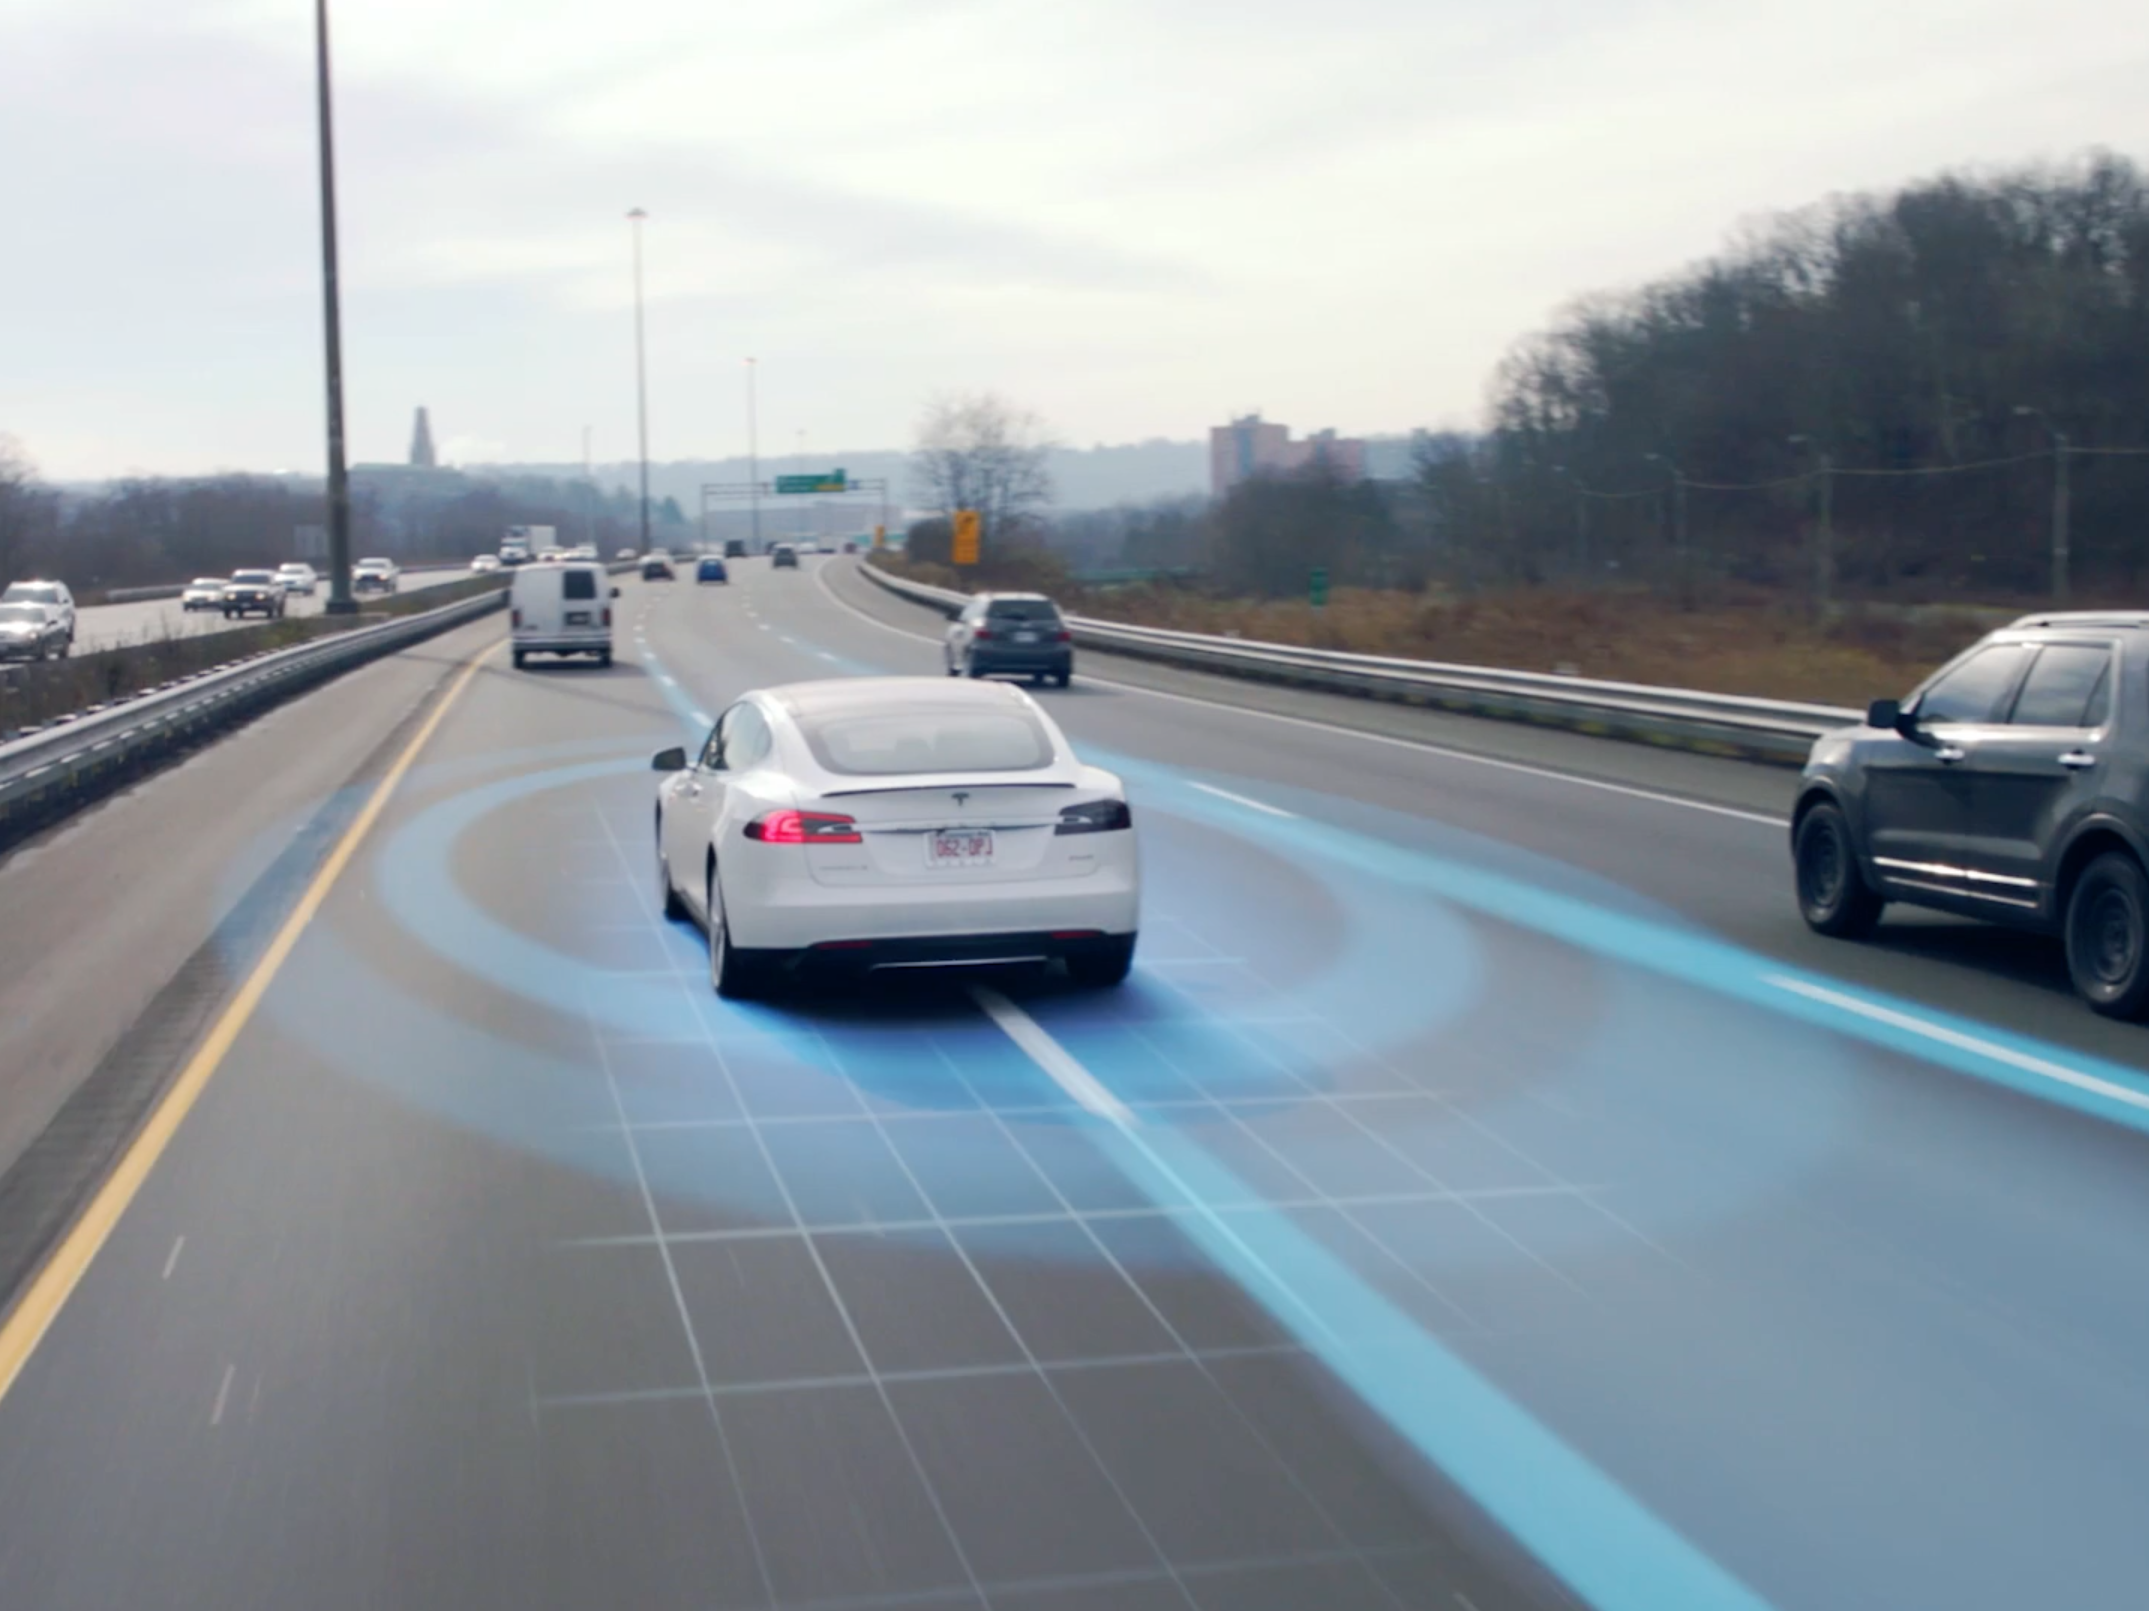
\includegraphics[height=.7\paperheight]{media/autonomous_car_real.png}};
        \node[right=of realAV] (notes) {%
            \begin{minipage}{.3\paperwidth}
                \begin{itemize}[<+(1)->]
                    \item Endanger people
                    \item Costs (financial and time)
                    \item Automation?
                    \item Reproducibility?
                \end{itemize}
            \end{minipage}
        };
        \pause%
        \node (simAV) at (realAV.east) {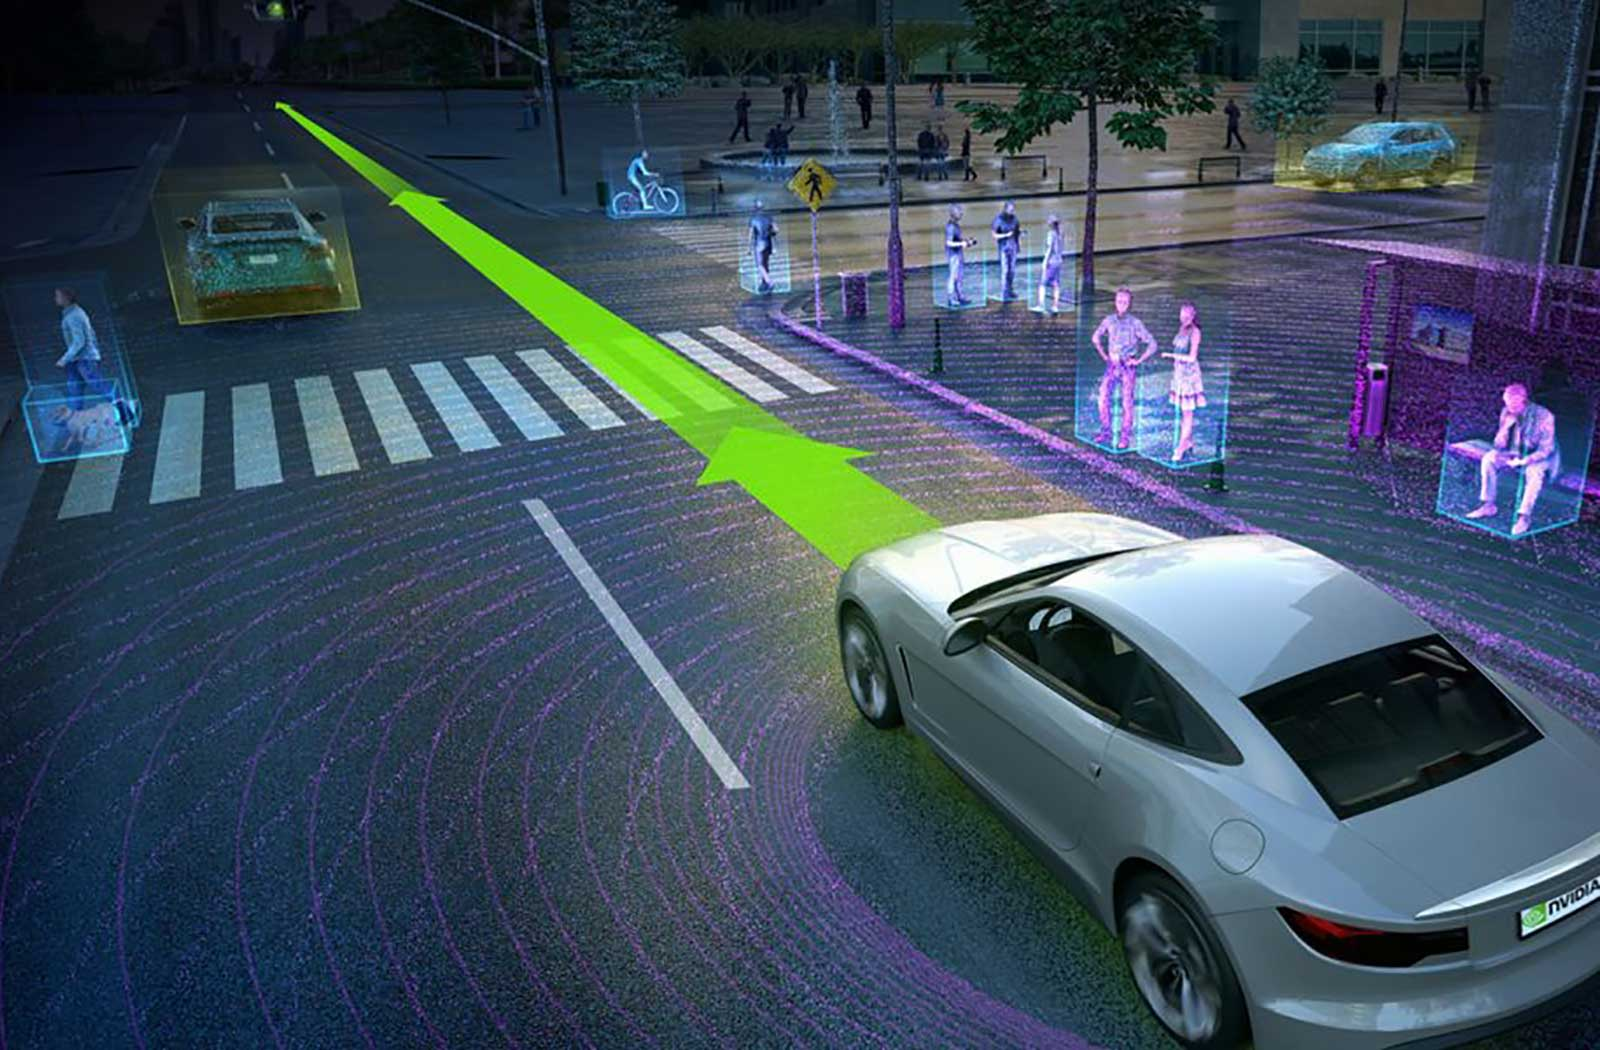
\includegraphics[height=.65\paperheight]{media/autonomous_car_simulation.jpg}};
    \end{tikzpicture}
\end{frame}

\begin{frame}[plain]
    \centering
    \Huge What about the environment?
    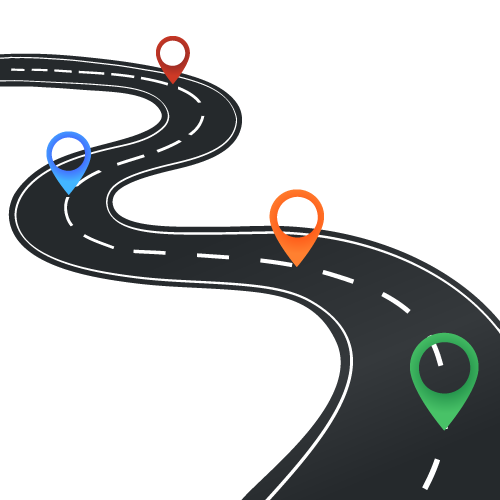
\includegraphics[height=.4\paperheight]{media/streets.png}
\end{frame}

\begin{frame}{Problem of Environment Description}
    \centering
    \begin{tikzpicture}
        \node (opendrive) {
\includegraphics[width=.4\paperwidth]{media/opendrive.png}};
        \node[below=0 of opendrive] (opencrg) {
\includegraphics[width=.4\paperwidth]{media/opencrg.png}};
        \node[below=0 of opencrg] (openscenario) {
\includegraphics[width=.4\paperwidth]{media/openscenario.png}};
        \pause%
        \node[right=0 of opencrg] (tedious) {
\includegraphics[height=.6\paperheight]{media/tedious.jpg}};
    \end{tikzpicture}
\end{frame}

\begin{frame}{Problem of Environment Description}
    \centering
    \begin{tikzpicture}
        \node (commonRoad) {
\includegraphics[width=.4\paperwidth]{media/commonRoad.png}};
        \node[right=of commonRoad] (notes) {%
            \begin{minipage}{.4\paperwidth}
                \begin{itemize}[<+(1)->]
                    \item Ignores physics
                    \item No realistic movements
                    \item Uncertainty
                    \item Only goal region criterion
                \end{itemize}
            \end{minipage}
        };
    \end{tikzpicture}
\end{frame}

\begin{frame}{Solution of Environment Description}
    \begin{itemize}[<+ (1)->]
        \item Describe static content as in simulator
            \pause%
            \(\Rightarrow\) Expected curvature
        \item Describe movements without\ldots
            \begin{itemize}
                \item \ldots tighten time and position
                \item \ldots explicit timing at all
                \item \ldots forcing to reach positions precisely
                \item \(\Rightarrow\) Rely on simulation physics
                \item \(\Rightarrow\) No need for redefining tests
            \end{itemize}
    \end{itemize}
\end{frame}

\begin{frame}[plain]
    \centering
    \Huge What about test criteria?\\
    
\includegraphics[height=.4\paperheight]{media/criteria.png}
\end{frame}

\begin{frame}{Problem of Criteria Description}
    \centering
    \begin{tikzpicture}
        \node (tooMuch) {
\includegraphics[width=.5\paperwidth]{media/tooMuchWork.jpg}};
        \pause%
        \node[right=of tooMuch] (connect) {
\includegraphics[width=.3\paperwidth]{media/connect.png}};
    \end{tikzpicture}
\end{frame}

\begin{frame}{Solution for Criteria Description}
    \centering
    \begin{tikzpicture}
        \node (adas) {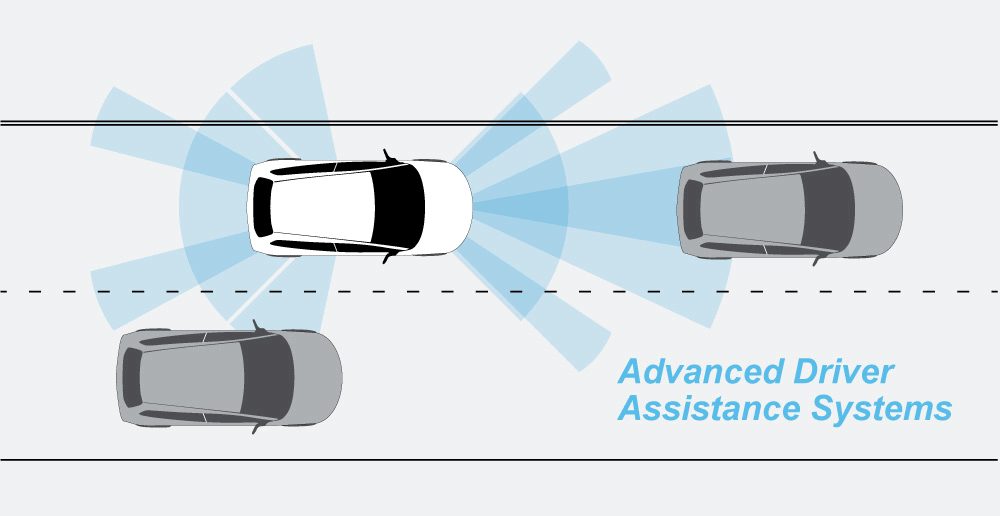
\includegraphics[height=.4\paperheight]{media/adas.png}};
        \pause%
        \node[right=of adas] (listOfAdas) {%
                \begin{minipage}{.4\paperwidth}
                    \begin{itemize}
                        \item Collision avoidance system
                        \item Emergency Brake Assist
                        \item Turning assistant
                        \item Cruise control
                        \item Intelligent speed adaptation
                        \item Adaptive cruise control
                        \item Active Brake Assistant
                        \item Lane centering
                        \item Lane departure warning system
                        \item Lane change assistance
                        \item Wrong-way driving warning
                    \end{itemize}
                \end{minipage}
            };
    \end{tikzpicture}
\end{frame}

\begin{frame}{Solution of Criteria Description}
    \centering
    % FIXME Mention success, failure, precondition separation?
    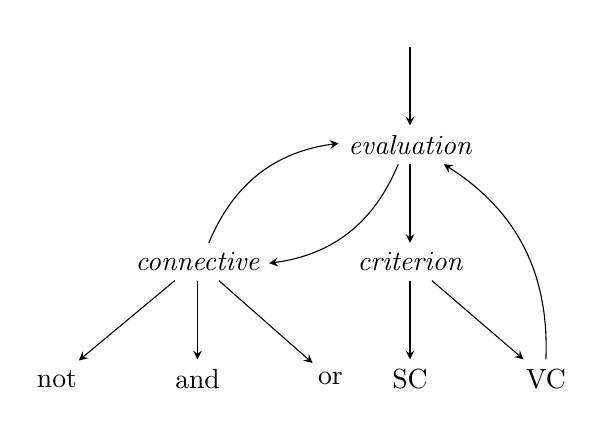
\begin{tikzpicture}[%
            ->,
            >=stealth
        ]
        \node (evaluation) {\itshape evaluation};
        \node[above=of evaluation] (start) {};
        \node[below=of evaluation] (criterion) {\itshape criterion};
        \node[left=of criterion] (connective) {\itshape connective};
        \node[below=of connective] (and) {and};
        \node[right=of and] (or) {or};
        \node[left=of and] (not) {not};
        \node[below=of criterion] (sc) {SC};
        \node[right=of sc] (vc) {VC};

        \path
            (start) edge (evaluation)
            (evaluation) edge (criterion)
            (evaluation) edge[bend left]  (connective)
            (connective) edge[bend left] (evaluation)
            (criterion) edge (sc)
            (criterion) edge (vc)
            (vc) edge[bend right] (evaluation)
            (connective) edge (not)
            (connective) edge (and)
            (connective) edge (or);
    \end{tikzpicture}
\end{frame}

\begin{frame}[plain]
    \centering
    \Huge What about training AIs?
    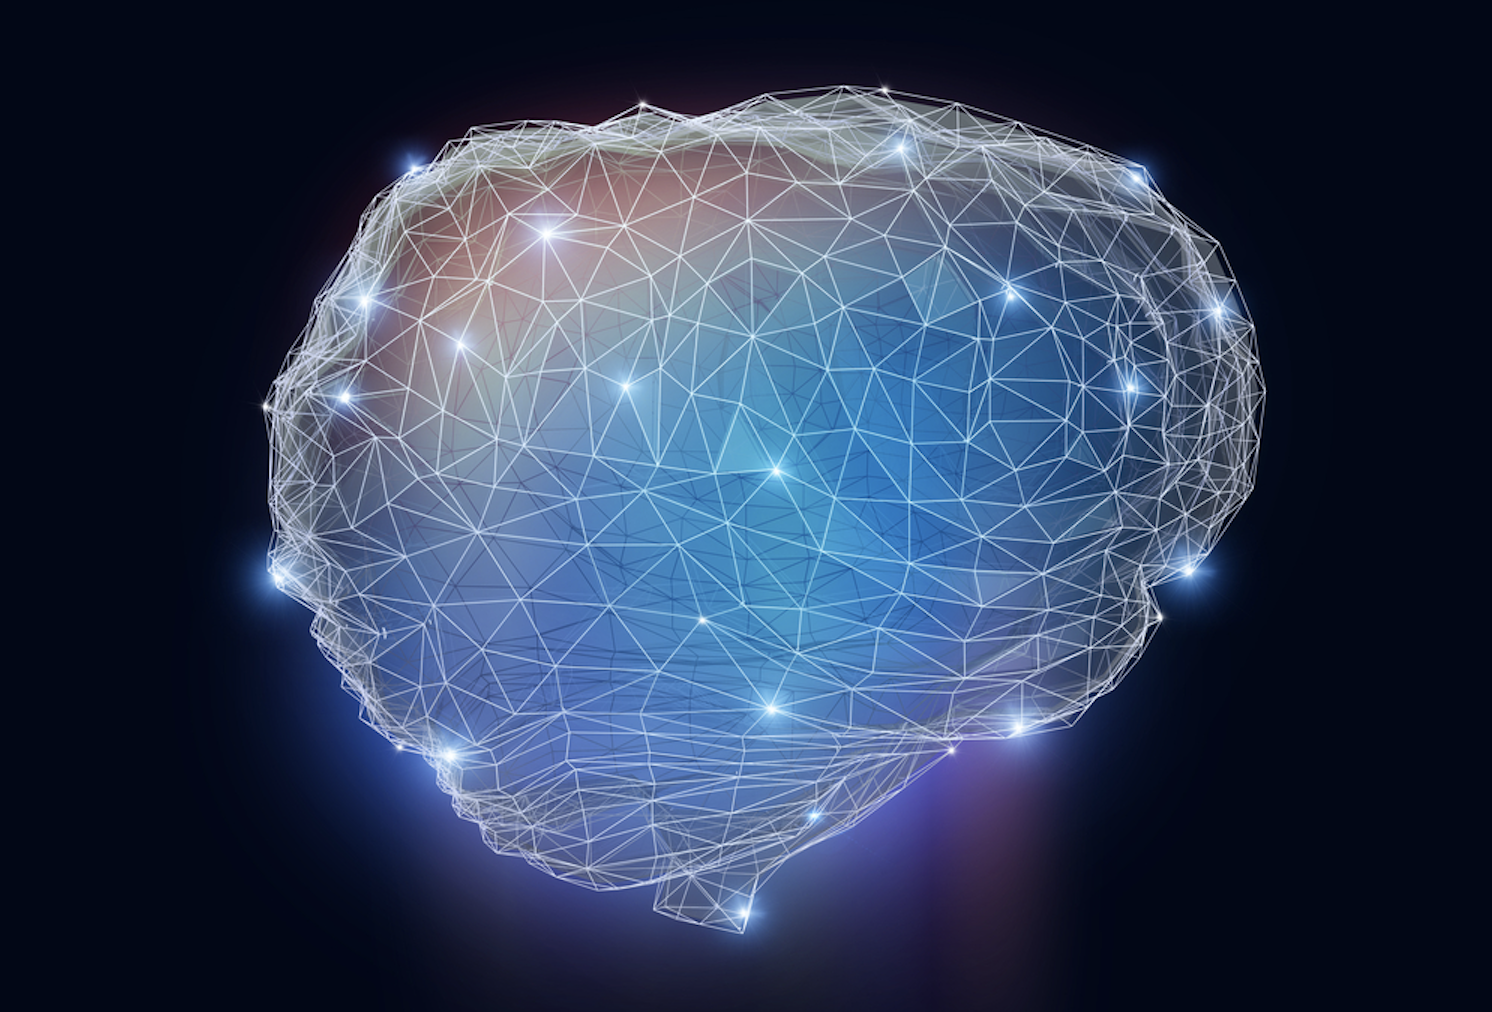
\includegraphics[height=.4\paperheight]{media/trainAI.png}
\end{frame}

\begin{frame}{Problems of Training AIs}
    \centering
    \begin{tikzpicture}
        \node (data) {
\includegraphics[width=.5\paperheight]{media/questionmark.png}};
        \pause%
        \node[right=of data] (collect) {
\includegraphics[height=.5\paperheight]{media/database.png}};
    \end{tikzpicture}
\end{frame}

\begin{frame}[plain]
    \centering
    \Huge What about the execution?
\end{frame}

\begin{frame}[plain]
    \centering
    \smartdiagram[flow diagram:horizontal]{%
        Verify criteria, Request AIs, Control, Start Resume, Pause
    }

\end{frame}

\begin{frame}{Evaluation}
    \centering
    \begin{tikzpicture}
        \pause%
        \node (seminar) {
\includegraphics[height=.7\paperheight]{media/seminar.jpg}};
        \pause%
        \node (ai) {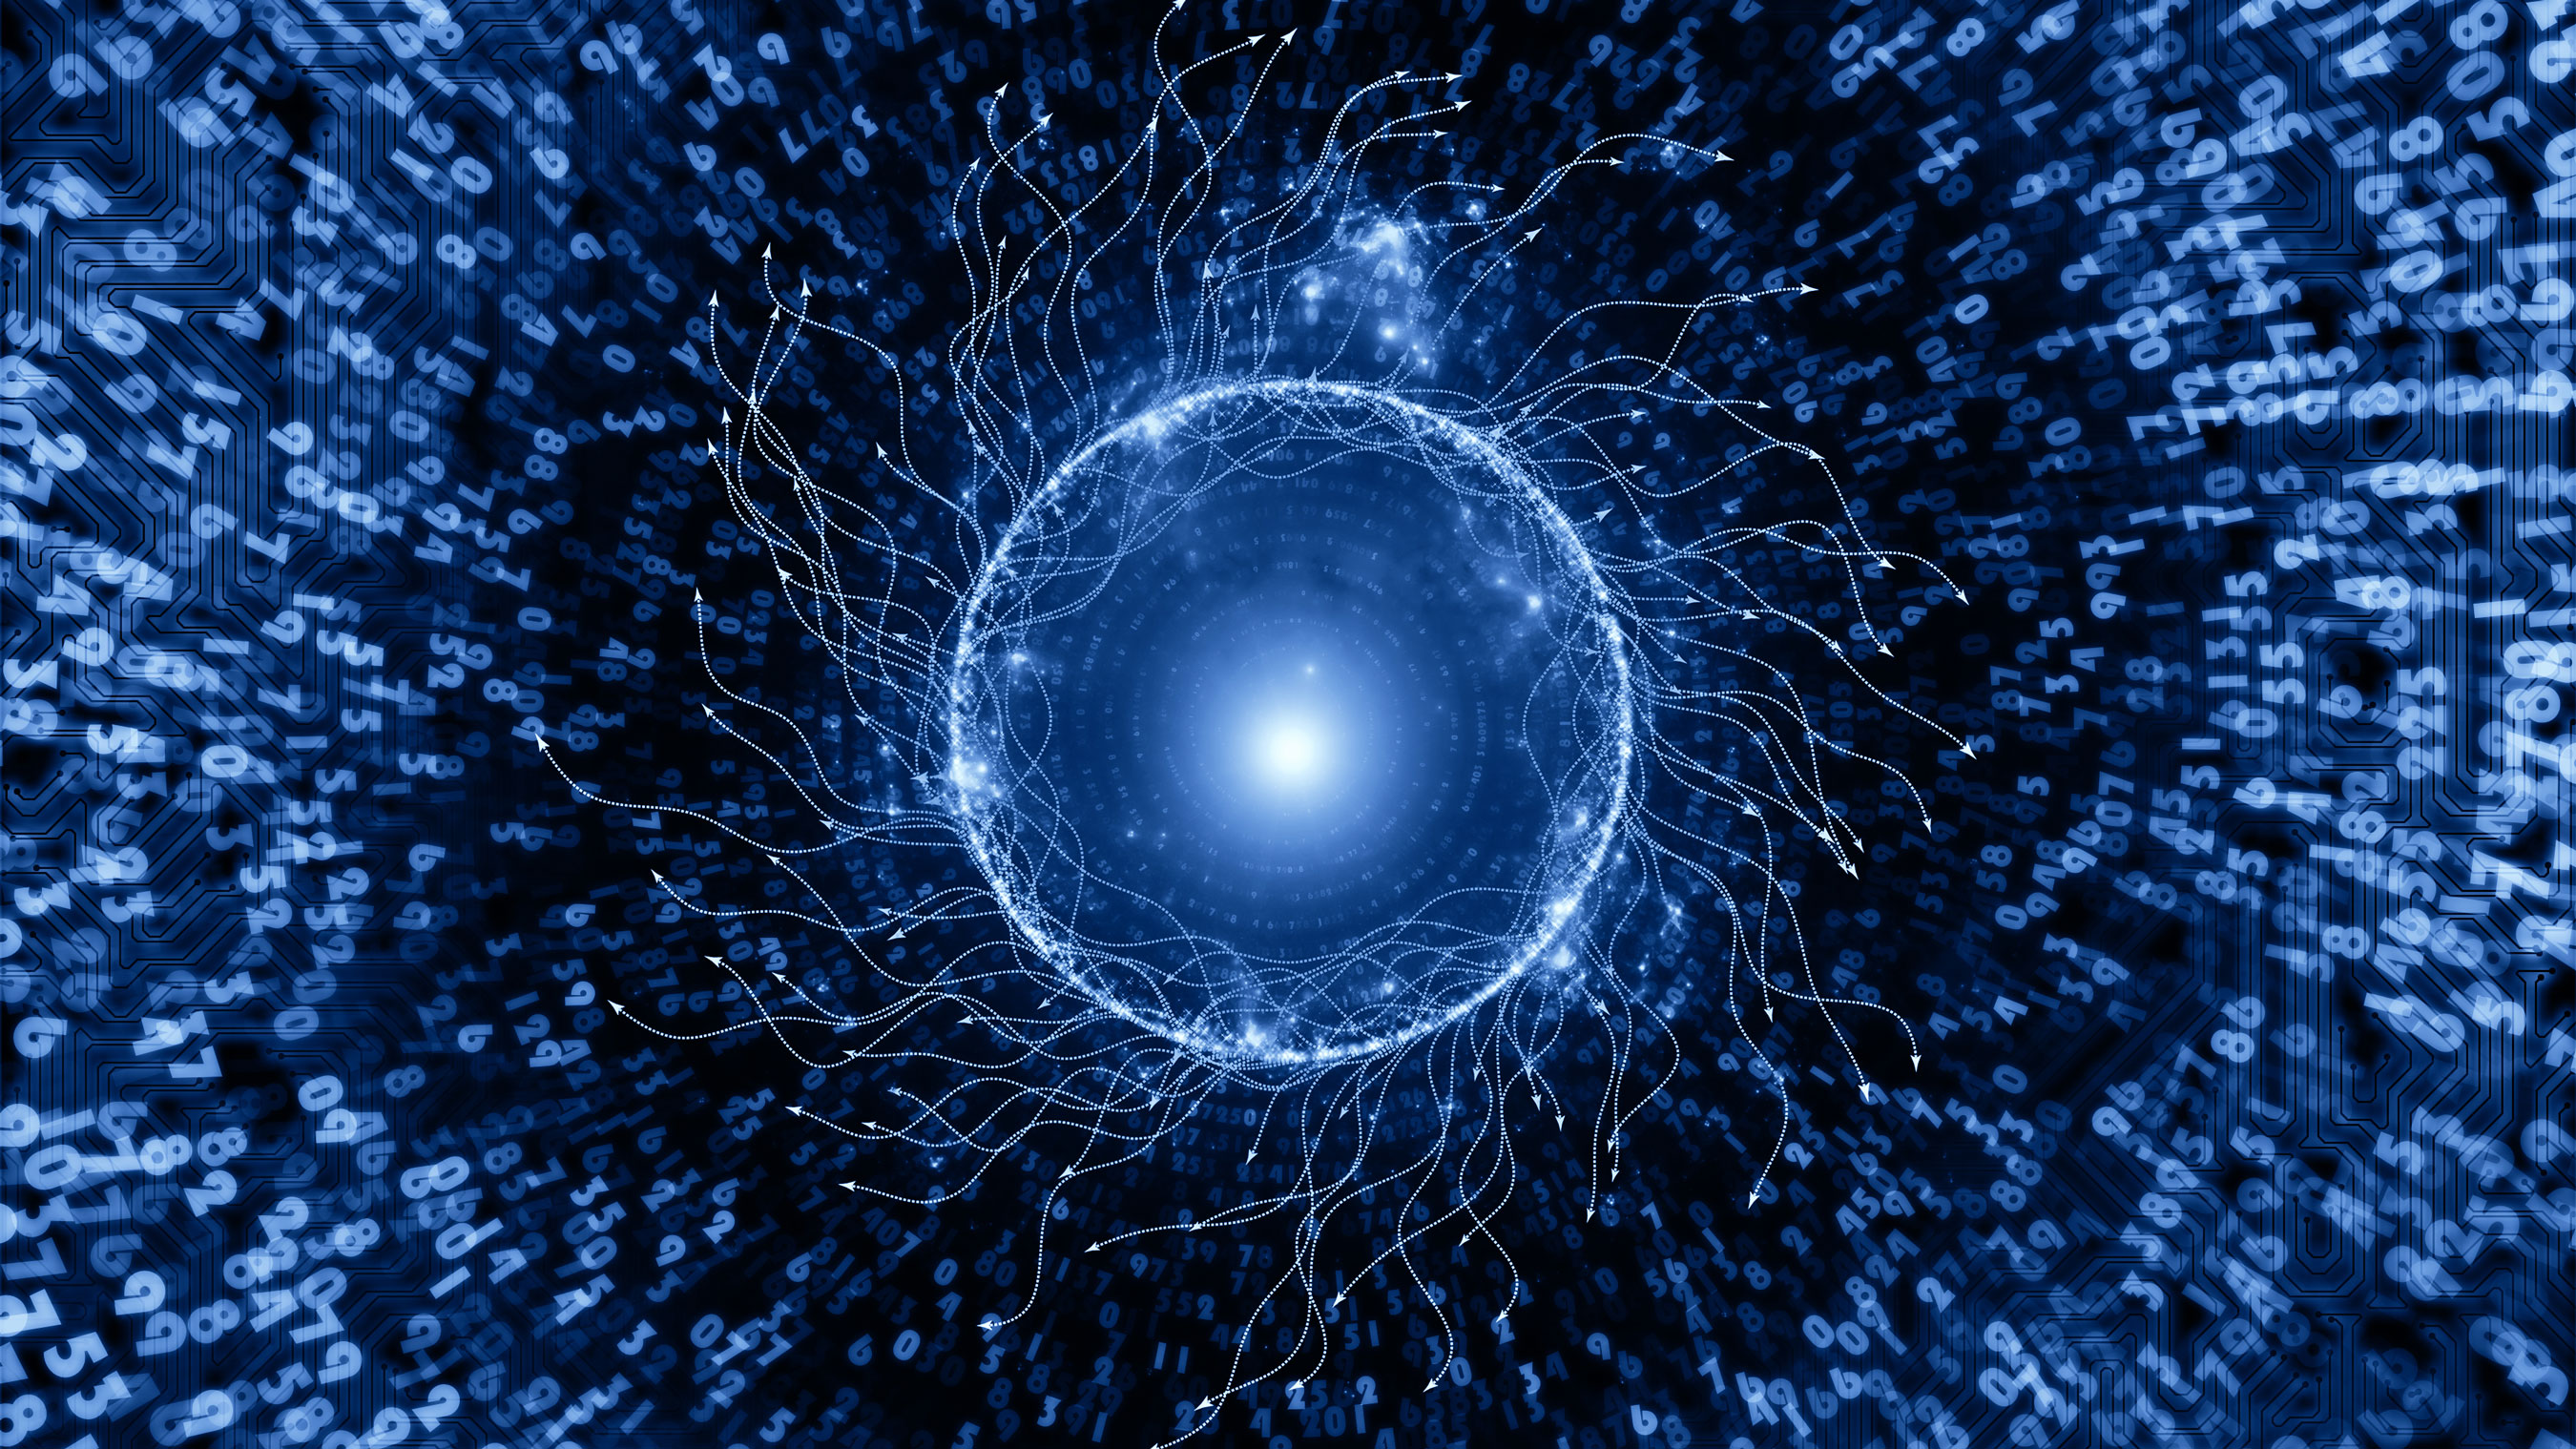
\includegraphics[width=.5\paperwidth]{media/ai.jpg}};
        \pause%
        \node (crash) {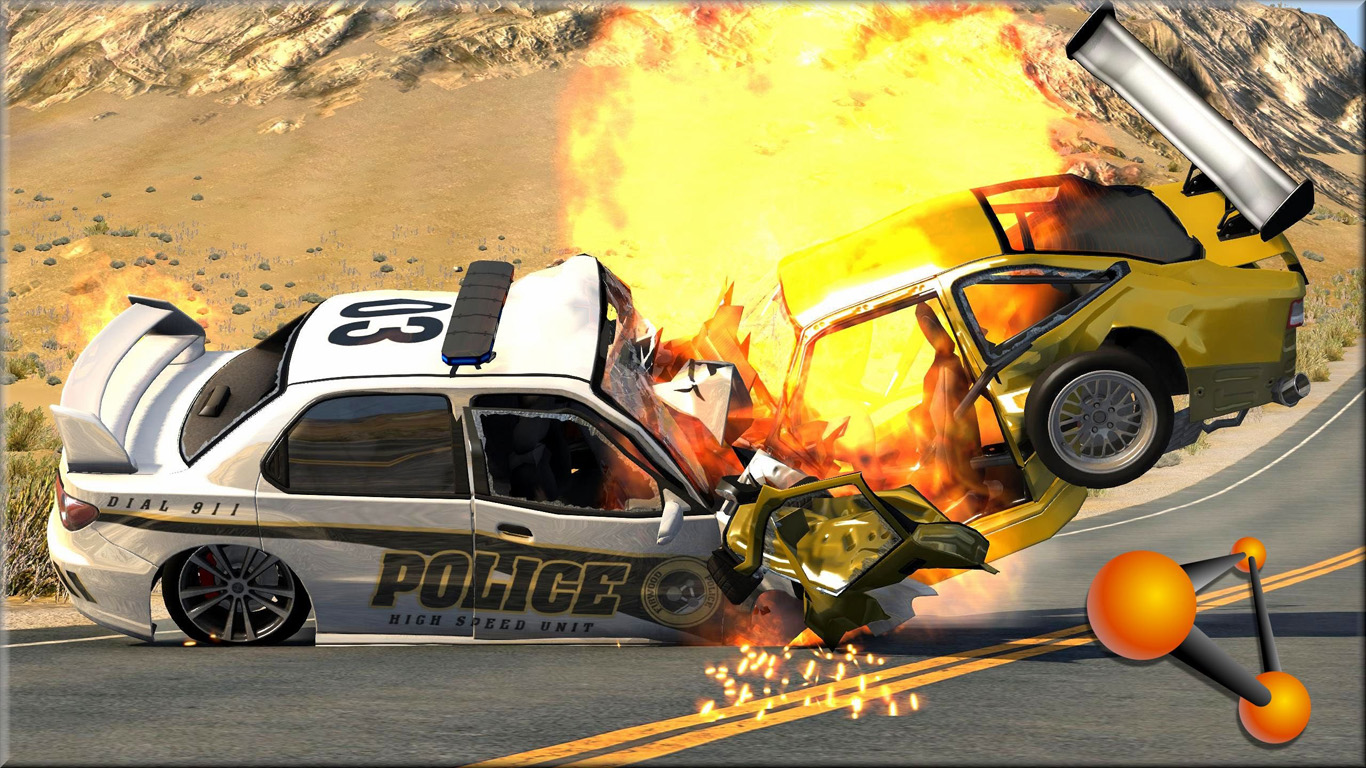
\includegraphics[width=.5\paperwidth]{media/crash.jpg}};
        \pause%
        \node (data) {
\includegraphics[width=.5\paperwidth]{media/data.jpg}};
        \pause%
        \node (prototype) {
\includegraphics[width=.6\paperwidth]{media/prototype.png}};
    \end{tikzpicture}
\end{frame}

\end{document}

